\documentclass{beamer}

\usepackage{subfigure}
\usepackage{graphicx}
\usepackage{sidecap}
\usepackage{caption}
%\usepackage{subcaption}
\captionsetup{compatibility=false}
\usepackage{appendixnumberbeamer}
\usepackage{amsmath}
% --
\usepackage{multirow}
\usepackage{xcolor}
\usepackage{setspace}
\usepackage{hyperref}
\usepackage{anyfontsize}

\beamertemplatenavigationsymbolsempty
\setbeamertemplate{footline}

\newenvironment{itemise} {\begin{itemize} \setlength{\itemsep}{0.2cm}} {\end{itemize}}
\usepackage[labelformat=empty]{caption}
\setbeamertemplate{sections/subsections in toc}[square]

%% COLORS
\definecolor{Gray}{gray}{0.9}
\definecolor{dblue}{rgb}{0.132,0.1,0.27}
\definecolor{mint}{cmyk}{1.0, 0.2, 0.6, 0.05}
\definecolor{ant}{cmyk}{0.5, 0.1, 0.0, 0.45}
\definecolor{lgray}{cmyk}{0.12, 0.0, 0.0, 0.17}
\definecolor{lred}{cmyk}{0.0, 0.9, 0.7, 0.0}


\usepackage{etoolbox}% http://ctan.org/pkg/etoolbox 
\usepackage{booktabs}

\newenvironment{literatur}{%
  \parskip2pt \parindent0pt \raggedright
  \def\lititem{\hangindent=0.5cm \hangafter1}}{%
  \par\ignorespaces}

\newcommand{\tb}[1]{{\color{blue}{\textbf{#1}}}}
\newcommand{\tm}[1]{{\color{mint}{\textbf{#1}}}}
\newcommand{\tr}[1]{{\color{red}{\textbf{#1}}}}
% Ilya: packages

\usepackage{tikz}
\usepackage{lmodern}
\usepackage{enumitem}

% Ilya: my commands

\newenvironment{mytemize}
{\vfill\itemize[nolistsep,itemsep=\fill,label=\color{blue}{$\triangleright$}]}
  {\enditemize}


\newenvironment{mynumerate}
{\vfill\enumerate[nolistsep,itemsep=\fill,label=\arabic*.]}
  {\endenumerate}

\newcommand{\hitem}[1]{
  {\color{blue}{$\triangleright$}} 
  {#1} 
  {\hfill}
}

\setlist[itemize]{label= \color{blue}{$\triangleright$}}
\setlist[enumerate]{label = \arabic*.}

\newcommand{\rarr}{$\Rightarrow$\ }



%\href{<Ziel>}{<Eingefasster Text>} 

%\logo{\includegraphics[height=0.7cm]{BdFlogo.eps}\hspace{300pt}\vspace{-5pt}}
%\logo{\includegraphics[height=0.8cm]{BdFlogo.eps}}
%\logo{\pgfputat{\pgfxy(-6.2,-0.5)}{\pgfbox[center,base]{\includegraphics[height=0.8cm]{BdFlogo.eps}}}}

%------------------------------------------------------------------------------------
% TITLE
%------------------------------------------------------------------------------------
\title[PSME]{Macroeconomics\\ Lecture 2 -- IS-TR-IFM, Intro to Dynamics} 
\author[I. Eryzhenskiy]{Ilya Eryzhenskiy}
\institute[BdF]{PSME Panth\'{e}on-Sorbonne Master in Economics}
\date[PSME macro]{Fall 2023}

%---BEGIN------------------------------------------------------------------------------
\begin{document}

\begin{frame}
  \maketitle
\end{frame}

\begin{frame}{Overview}
  \tableofcontents
\end{frame}

\section{Exchange rates \& goods market (IS); capital flows (IFM)}

\begin{frame}
\tableofcontents[currentsection]
\end{frame}

\begin{frame}{Foreign exchange as a market}
  \begin{figure}
	\centering
	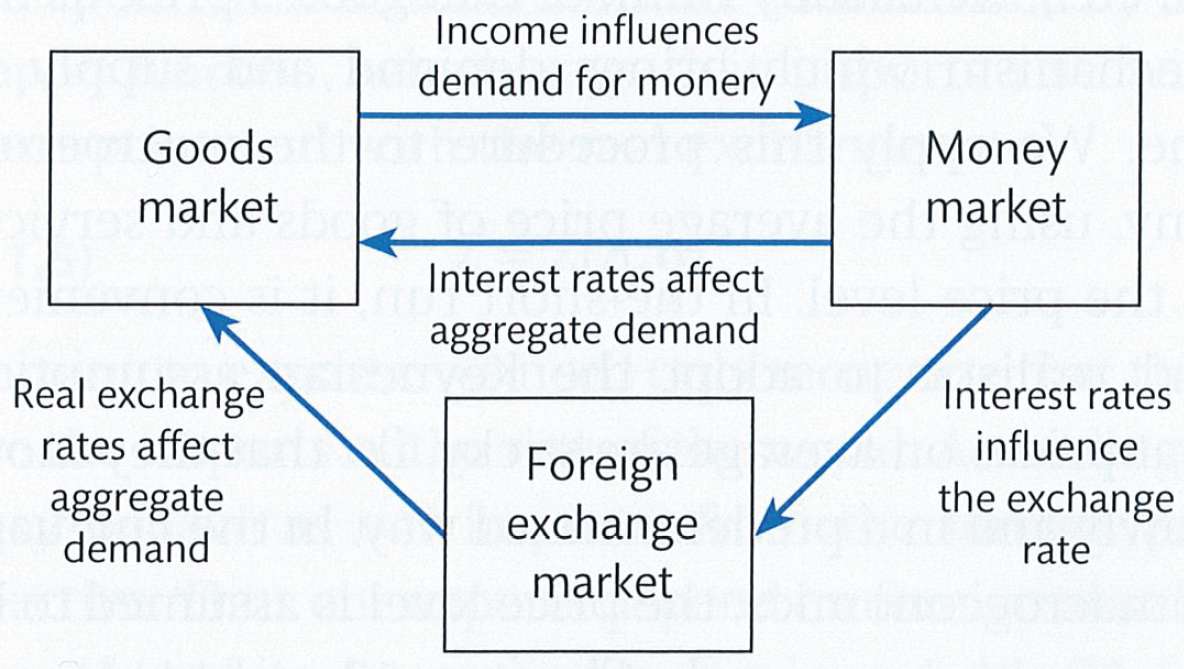
\includegraphics[width=0.8\textwidth]{FIGURES/6_GE.png}
  \end{figure}
\begin{minipage}{1.0\columnwidth}
\tiny	
%	\textbf{Note.} The Figure shows the average behaviour of variables around cyclical peaks in eight countries.\\
\textbf{Source.} Burda and Wyplosz (2017), Figure 10.2.\\
\end{minipage}
\end{frame}

\begin{frame}{%
\protect\hypertarget{lecture-overview-opening-up-is-tr-and-ad-as}{%
Lecture overview: opening up IS-TR}}

 We already introduced \tb{trade balance}, but assumed it is null in equilibrium. This lecture:
\begin{mynumerate}

 
\item
  TB is nonzero in equilibrium and it is driven by \tb{real exchange rate}

  \begin{mytemize}
  \item
	Real exchange rate \textbf{shifts} IS
  \end{mytemize}
  \item Economy also open to \tb{capital flows}

  \begin{mytemize}
   
  \item
    \tb{International Financial Markets (IFM) line} \rarr IS-TR-IFM model
  \end{mytemize}
%\item
  %Medium run (AD-AS): inflation affects \tb{real exchange rate} 

%\item
  %Long run: \tb{purchasing power parity} affects inflation and exchange rate 
\end{mynumerate}
\vfill
Equilibrium analysis must be done separately for \tb{fixed} and \tb{flexible} exchange rate regimes.
%\vfill
%AS is same as in closed economy (simplification).

\end{frame}

\begin{frame}{%
\protect\hypertarget{exchange-rates-quick-overview}{%
Exchange rates -- quick overview}}

\tm{Nominal} vs. \tb{real} exchange rates:

\begin{mytemize}
 
\item
  \tm{Nominal} exchange rate -- number of units of one currency per unit
  of another \(\Leftrightarrow\) \textbf{relative price of monies}

  \begin{mytemize}
   
  \item
    Can be expressed in units of foreign currency per unit of domestic
    or vice versa
  \item
    Example: EUR-JPY exchange rate is 140 JPY for 1 EUR
  \end{mytemize}
\item
  \tb{Real} exchange rate (RER) - ratio of foreign consumption basket value to
  domestic consumption basket value \(\Leftrightarrow\) \textbf{relative
  price of consumption}
\end{mytemize}

Using \(S\) as \tm{nominal} exchange rate (number of units of foreign
currency per unit of domestic), \(P\) the domestic and \(P^*\) the
foreign price level, define the \tb{real} exchange rate \(\sigma\) as:
\[ \sigma = \frac{S \cdot P}{P^*}\]

\end{frame}

\begin{frame}
\tableofcontents[currentsection]
\end{frame}
%\begin{frame}{IS curve in open economy}
%
%  IS obtained from equality of total goods available (left hand side) and all the uses of the goods (right hand side):
%\begin{align*}
%  Y + \underbrace{Z}_{\text{imports}}=C+I+G+\underbrace{X}_{\text{exports}} 
%\end{align*}
%Re-arranging, we get:
%\begin{align*}
%  Y=C+I+G+\underbrace{(X-Z)}_{\text{primary current account (PCA)}}
%\end{align*}
%\end{frame}

%\begin{frame}{Primary current account}
%
%\tm{Import function}
%\begin{equation}
%Z = Z(\underset{+}{Y},\underset{+}{\sigma}) \tag{11.5}
%\end{equation}
%\begin{itemize}
%  \item Increases in income (proportional to disposable income or to consumption), example: $Z = z \cdot C = z \cdot c \cdot (Y-T))$
%\item Increases with real exchange rate appreciation ($\sigma \uparrow$, where $\sigma=SP/P^*$), domestic goods relatively expensive \rarr import$\uparrow$
%\end{itemize}
%
%\tm{Export function}
%\begin{equation}
%X = X(\underset{+}{Y^*},\underset{-}{\sigma}) \tag{11.6}
%\end{equation}
%\begin{itemize}
%  \item \textbf{demand-driven exports}: foreign income $\Rightarrow$ foreign demand. Domestic income/production not relevant!
%\item with real exchange rate appreciation ($\sigma \uparrow$), domestic goods relatively expensive \rarr less exports
%\end{itemize}
%
%\tb{Primary Current Account (PCA)} or Net Exports:
%\begin{align*}
%PCA = &X(\underset{+}{Y^*},\underset{-}{\sigma})-Z(\underset{+}{Y},\underset{+}{\sigma}) \\
% =	 & PCA(\underset{-}{Y},\underset{+}{Y^*},\underset{-}{\sigma})   
%\end{align*}
%
%\end{frame}

%\begin{frame}{Keynesian multiplier in open economy}
%  Assume linear functions: $C = c\cdot (Y-T)$ \\ $Z = z\cdot C = z \cdot c \cdot (Y-T)$ \\
%Consider an increase in government expenditure, $\Delta G$
%\begin{itemize}
%\small
%\item $DD\uparrow$, firms will produce more, ..., $Y\uparrow$
%\item \tb{Multiplier}: how much output changes $\Delta Y$, relative to shock $\Delta G$
%\item firms will increase production by $\Delta G$
%\item this generates new income, thus $C\uparrow$ but $PCA\downarrow$, $\Delta DD = c \Delta G - z c \Delta G = c(1-z)\Delta G$
%\item[$\rightarrow$] $Y\uparrow, C\uparrow, PCA\uparrow, Y\uparrow\dots$ -- recall staircase graph
%\item additional spending $\Delta C + \Delta PCA$ is smaller than $\Delta G$ due to \textit{leakages}, so $\Delta Y_2< \Delta Y_1$
%\item leakages in open economy: savings, \tr{imports}, taxes (if proportional)
%%\item $\Delta Y/\Delta G >1$
%\end{itemize}
%{
%\begin{align*}
%\Delta Y =& \Delta G + c(1-z)\Delta G + c^2(1-z)^2\Delta G + ...+c^n(1-z)^n\Delta G \\
%	&= \underbrace{\alert{\frac{1}{1-c(1-z)}}}_{\text{multiplier}>1} \Delta G
%\end{align*}
%}
%\end{frame}


%---FRAME------------------------------------------------------------------------------
\begin{frame}{Open economy IS}
 How does a change of real exchange rate $\sigma$ affect IS?
 \begin{mytemize}
\item RER appreciation \rarr more imports, less exports \rarr for a given interest rate, goods market equilibrium has lower $Y$ because of lower aggregate demand
 \end{mytemize}
\begin{align*}
Y = C(\underset{+}{\Omega}, \underset{+}{Y-T}) + I(\underset{-}{r}, \underset{+}{q}) + G + TB(\underset{-}{Y},\underset{+}{Y^*},\underset{-}{\sigma})
\end{align*}
\begin{align*}
  \underbrace{Y - C(\Omega, Y-T) -  TB(Y,Y^*,\sigma)}_{\text{increases in}\ Y,\ \sigma}=  I(\underset{-}{i - \pi^e}, q) + G 
\end{align*}
\begin{mytemize}
\item Mathematics: left hand side increasing in both $Y$ and $\sigma$ \rarr for a fixed right hand side, $Y\downarrow$ when $\sigma\uparrow$ for equation to hold
\item[\rarr] when $\sigma\uparrow$, $Y\downarrow$ for fixed $i$ \rarr \tr{IS shifts left} in $(Y, i)$ space. 
\end{mytemize}
\end{frame}

\begin{frame}{What are capital flows?}
  Here, a financial notion of capital is used: including any assets $+$ currency. \\
  \vfill
  \tb{Capital flows} are cross-country operations with capital. They are registered in the \tb{financial account} of Balance of Payments.
Examples of capital flows: 
\begin{mytemize}
\item Foreign exchange market
\item Lending/borrowing with non-resident
\item Foreign direct investment
\end{mytemize}
%\vfill
%Policy of capital movement restriction: \tr{capital controls}
%\begin{mytemize}
%\item Goes against orthodox economic theory/finance, but\dots
%\item Actively used by China \rarr relevant for understanding world economy
%\item \tr{Not studied} in this lecture
%\end{mytemize}
\end{frame}

\begin{frame}{International financial market: capital flows}
  
  We assume a \tb{small open economy} with free capital flows (no \emph{capital controls}):
  \begin{mytemize}
  \item Recall small open economy definition: country does not influence international prices
  \item \dots in particular, international nominal interest, $i^*$
  \item free capital flows \rarr no \tb{arbitrage} possibilities between domestic and foreign assets, \textbf{returns are equalized}: $i = i^*$
  \item[\rarr] a new condition in the $(Y, i)$ space: a horizontal IFM line
  \end{mytemize}
\end{frame}

\begin{frame}{Economy off IFM line -- exchange rate regime matters}
  What happens after capital inflows/outflows? What consequences for IS, TR?% \rarr for AD?
  \vfill
  $\rightarrow$ answers depend on \tb{exchange rate regime}
  \begin{mytemize}
  \item Under \tb{fixed exchange rate regime}, CB must prevent changes in \tb{nominal exchange rate}
	\begin{mytemize}
	\item Taylor Rule and money supply change such that $i = i^*$ again
	\end{mytemize}
  \item  Under \tb{flexible exchange rate regime}, central bank (CB) does not react, nominal (and real) exchange rate changes \rarr IS shifts 
	\begin{mytemize}
	\item IS \textbf{less influenced by demand shocks} than in closed economy or under fixed exchange rate 
	\end{mytemize}
  \end{mytemize}
\end{frame}

\section{Fixed exchange rate regime}
\begin{frame}
\tableofcontents[currentsection]
\end{frame}

\subsection{IS-(TR)-IFM equilibrium}
\begin{frame}{%
\protect\hypertarget{fixed-exchange-rate-in-is-tr}{%
Fixed exchange rate}}

\begin{mytemize}

\item Central bank fixes the nominal exchange rate: $S = \bar S$ \rarr $\sigma = \frac{\bar S P}{P^*}$

\item This is done via \tb{foreign exchange interventions} -- purchase/sale of foreign currency by the CB 

  \item
  Change of CB \textbf{assets} must be coupled with changes of
  \textbf{liabilities} -- the money supply

\end{mytemize}
\vfill
Simplified structure of a central bank balance sheet: 
$$\underbrace{\text{Domestic Credit}+\text{Foreign exchange reserves}}_{\text{Assets}} = \underbrace{\text{Money supply}}_{\text{Liabilities}}$$
\vfill
Foreign exchange interventions change the reserves \rarr change in money supply
\end{frame}
\begin{frame}{Fixed exchange rate, TR and IFM lines}
    
\begin{mytemize}
  \item
  Loss of control over $i$ because of capital flows:
  $i = i^*$; choice of money supply by the CB dictated by exchange rate. Taylor Rule is \textit{de facto} given up
\item[\rarr]
  Graphically, TR is no longer determining equilibrium: 
\item
  The horizontal IFM line in (i, Y) space determines equilibrium instead
  of TR 
  \item Behind the scenes, the foreign exchange interventions and corresponding changes in money supply make TR move wherever the new equilibrium is
\end{mytemize}
\vfill  We will consider different types of shocks in this IS-(TR)-IFM
  framework.
\end{frame}

\begin{frame}{%
\protect\hypertarget{demand-shock-e.g.government-spending}{%
Demand shock (e.g.~government spending)}}

\end{frame}


\begin{frame}{
Devaluations/revaluations: explanation}

\end{frame}

\begin{frame}{%
Devaluations/revaluations --- changes of $\bar S$}

\begin{mytemize}

\item
  IS moves as explained before
\item
  Central bank must adapt monetary policy -- TR shifts
\item
  Behind the scenes -- central bank buys or sells foreign currency to
  keep S fixed -- \tb{foreign exchange interventions}

\end{mytemize}

\end{frame}

\begin{frame}{%
\protect\hypertarget{international-financial-shock-shift-of-ifm}{%
International financial shock -- shift of IFM}}

\begin{columns}
\column{0.35\textwidth}
An increase in world interest rate is contractionary for fixed exchange rate economies\\
\vspace{3cm}
Very relevant shock for 2022-2023: US rate went from 0.33 to over 5 p.p.
\column{0.65\textwidth}
\end{columns}

\end{frame}


\section{Flexible exchange rate regime}
\begin{frame}
\tableofcontents[currentsection]
\end{frame}
\subsection{(IS)-TR-IFM equilibrium}
\begin{frame}{%
\protect\hypertarget{flexible-exchange-rate}{%
Flexible exchange rate}}

\begin{mytemize}
 
\item
  Monetary policy is again independent
\item
  Aggregate demand has additional source of variation: real exchange rate changes through \tb{nominal} exchange rate reaction to \tb{capital flows}
\item Position of IS becomes endogenous; TR and IFM determine equilibrium: (IS)-TR-IFM
\end{mytemize}

\end{frame}

\begin{frame}{%
\protect\hypertarget{monetary-policy-shock-graph}{%
Monetary policy shock with flexible exchange rates}}
\vspace{-5cm}
Monetary policy \textit{de facto} operates through \tr{exchange rate} and \tr{not interest rate}

\end{frame}

\begin{frame}{%
\protect\hypertarget{demand-shock-e.g.government-spending}{%
Demand shock (e.g.~government spending) with flexible exchange rates}}
\vspace{-5cm}
Exchange rate acts as \tr{stabilizer} of aggregate demand
 

\end{frame}

\begin{frame}{%
\protect\hypertarget{international-monetary-shock}{%
International monetary shock}}
\vspace{-5cm}
An increase in foreign interest rate is \tr{expansionary} --\\
\tr{opposite} of \tr{fixed} exchange rate case.

\end{frame}

\begin{frame}{%
\protect\hypertarget{international-monetary-shock-ii-beggar-thy-neighbour-effect}{%
International monetary shock II: beggar-thy-neighbour effect}}

\begin{mytemize}
 
\item
  Suppose a large foreign economy lowers $i^*$ in expansionary monetary
  policy
\item
  How does equilibrium change? \textcolor{mint}{Draw an (IS)-TR-IFM plot}
\item
  Domestic $i$ relatively high \rarr capital inflow \rarr real exchange
  rate appreciation \(\sigma \uparrow\)
\item
  IS moves to the left, equilibrium output lower
\item
  Foreign expansionary policy at the expense of neighbours' output. A critique of quantitative easing policies in developed economies post-2008, from smaller economies' perspective
\end{mytemize}

\end{frame}


%
%\section{More on exchange rate regimes}
%\begin{frame}
%\tableofcontents[currentsection]
%\end{frame}

\begin{frame}{Recap: trade-offs of exchange rate regimes}
  Each exchange rate regime presents pros and cons. Seen in this lecture: 
  \begin{mytemize}
  \item \tb{Fixed} exchange rate regime:
	\begin{mytemize}
	\item  facilitates trade of goods, services and assets, \tr{but}
	\item eliminates independent monetary policy (control over $i$)
	\item not necessarily bad, e.g. if CB has \tb{commitment} problems leading to high inflation
	\end{mytemize}
  \item \tb{Flexible} of floating exchange rate regime:
	\begin{mytemize}
	\item creates problems in trade, \tr{but}
	\item allows for monetary policy independency $+$ acts as absorber of demand shocks
	\end{mytemize}
  \end{mytemize}
  Important issues of \tb{foreign exchange reserves} management not covered in lecture -- another argument against fixed regimes when CB is not trusted by public.
\end{frame}

\begin{frame}{Beyond fixed vs. flexible: IMF classification}
  Many regimes exist as countries trade off benefits and costs of fixed and flexible exchange rates.
  \begin{figure}[ht]
	\hspace{-0.5cm}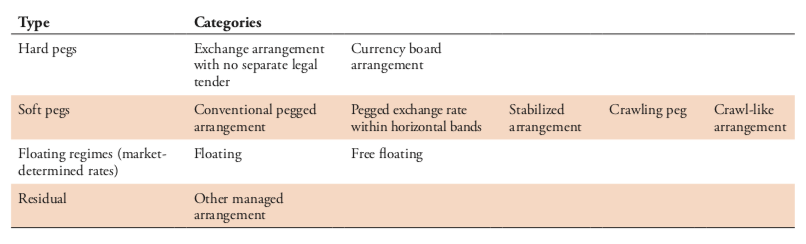
\includegraphics[width = 1.28\textwidth]{FIGURES/IMF_exchange_rate_regimes}
  \end{figure}
	\tiny Source: IMF Annual report on exchange arrangements and exchange restrictions (2021).
\end{frame}

\section{Introduction to Dynamics: Multiplier-Accelerator}
\begin{frame}
\tableofcontents[currentsection]
\end{frame}

\begin{frame}{Multiplier-Accelerator model}
  \begin{mytemize}
  \item A simple Keynesian model of the goods market that generates endogenous business cycles
	\item \tr{NOT} the way we think about cycles today\dots
  \item[\dots] but is a useful introduction to \tr{dynamics}
  \end{mytemize}
  \vfill
  A closed economy model of goods market. 3 equations:
  \begin{mynumerate}
  \item  Consumption depending on \textbf{last period} income
  \item  Investment depending on \textbf{growth of} income in \textbf{last period} --- the \tb{accelerator} assumption
  \item Goods market equilibrium (IS)
  \end{mynumerate}
\end{frame}

\begin{frame}{Multiplier-Accelerator accelerator model}{Variables}

Time runs from $t=1$ to $\infty$
\begin{mytemize}
\item
  \(\{C_t\}\) --- sequence of consumption
\item
  \(\{I_t\}\) --- sequence of investment, the key
  \textit{endogenous} variable
\item
  \(\{Y_t\}\) --- sequence of GDP
\item
  \(\{G_t\}\) --- sequence of of 
\textbf{exogenous} government expenditures. We will consider constant expenditure mostly, but it can be a source of shocks
\end{mytemize}

\end{frame}

\begin{frame}{Model structure}

The model combines the consumption function

 \[
C_t = a Y_{t-1} + \gamma 
\]

with the investment accelerator

 \[
I_t = b (Y_{t-1} - Y_{t-2})
\]

and the goods market equilibrium

 \[
Y_t = C_t + I_t + G_t 
\]

\begin{mytemize}
 
\item
  The parameter $a$ is \tb{mpc} (past income assumed most relevant for decisions -- this assumption is given up by modern models)
\item
  The parameter \(b > 0\) is the investment accelerator coefficient:
  investment in physical capital is done when GDP is increasing and
  \tb{disinvestment} is done when it is decreasing
\end{mytemize}

\end{frame}

\begin{frame}{Solution: a difference equation}

  Combining the three equations:
  $$
Y_t = (a+b) Y_{t-1} - b Y_{t-2} + (\gamma + G_t)
$$
\vfill
Defining new coefficients gives compact form: assume $\rho_1 = (a+b)$ and $\rho_2 = -b$, then:
$$
Y_t = \rho_1 Y_{t-1} + \rho_2 Y_{t-2} + (\gamma + G_t) 
$$
\vfill
Assuming initial values to generate the sequence $
\{Y_t\}$ for $ t=0, \ldots, T $:

$$
Y_{-1} = \bar Y_{-1}, \quad  Y_{-2} = \bar Y_{-2}
$$

When simulating the model, set $(a,b)$ so that starting from
$(\bar Y_{-1}, \bar Y_{-2})$,  ${Y_t}$ converges to
a constant value under constant $G$: this is the \tb{steady state} of the economy

\end{frame}

\begin{frame}{Model dynamics: no shocks}
\begin{figure}
    \centering
    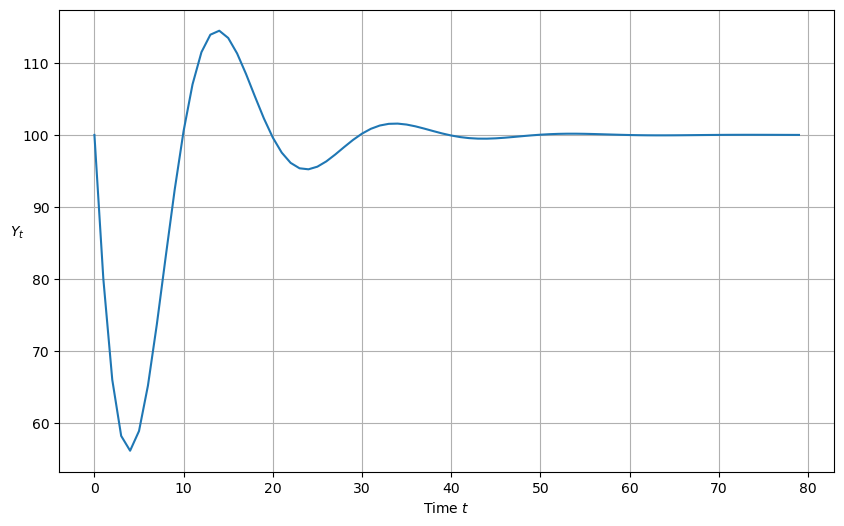
\includegraphics[width=0.8\textwidth]{FIGURES/Samuelson_Y.png} \\
    \tiny Source: \href{https://python.quantecon.org/samuelson.html}{QuantEcon (link)}
\end{figure}
\end{frame}

\begin{frame}{Why the cycles? Intuition}
   What if there was no investment in the model? Then:  
   $$Y_t =  a Y_{t-1} + \gamma + G$$
   where government expenditure is again assumed constant: $G_t = G$) \\
   \vfill
    The steady state level of $Y$ is easy to compute: $$Y^{ss} = a Y^{ss} + \gamma + G \Rightarrow Y^{ss} = \frac{\gamma + G}{1-a}$$ and we get that $Y_t - Y^{ss} = a (Y_t - Y{ss})$ \textcolor{mint}{(verify this)} \\
    \rarr the difference between $Y_t$ and $Y^{ss}$ decreases over time \rarr $Y_t$ converges, no cycles \\
    \vfill 
    In the full model, the accelerator $I_t = b (Y_{t-1} - Y_{t-2})$ makes $Y_t$ \textbf{overshoot} the steady state, but the consumption dynamics makes it converge back after each overshoot
\end{frame}

\begin{frame}{Why the cycles? Illustration}
    
\end{frame}

\begin{frame}{Why the cycles? Math}
Let's solve the full model in a \tb{linear state space form} using matrices \\
\vfill Define a \tb{state vector} $x_t = \begin{pmatrix}
    Y_{t-1} \\ Y_{t-2}
\end{pmatrix}$. \\ \vfill We can write the dynamical equation $Y_t = a Y_{t-1} + b (Y_{t-1}-Y_{t-2}) + \gamma + G$ in a matrix form:
$$x_{t+1} = A x_t + d$$
where $A = \begin{pmatrix}
    a+b & -b \\ 1 & 0
\end{pmatrix}$
\vfill
Model dynamics is then determined by \tr{eigenvalues} of $A$
\end{frame}

\begin{frame}{Why the cycles? Math}
  With eigenvalues $\lambda_1, \lambda_2$, the dynamics of $Y_t$ given by:
  $$
Y_t = \lambda_1^t c_1 + \lambda_2^t c_2
$$
where $ c_1 $ and $ c_2 $ are constants on parameters and initial conditions.
initial conditions and on $ \rho_1, \rho_2 $.
\vfill
When the eigenvalues are complex, can represent them in polar form $
\lambda_1 =  r e^{i \omega}, \  \lambda_2 = r e^{-i \omega}
$ and rewrite the solution as follows (\alert{not necessary to memorize!}):
$$
  Y_t =  (c_1 + c_2) r^t \cos(\omega t) + i (c_1 - c_2) r^t \sin(\omega t)
$$
Parameters and intital conditions chosen such that $c_1+c_2$ real, $c_1-c_2$ complex, so $Y_t$ real and has a form:
$$Y_t = 2 v r^t  \cos (\omega t + \theta),$$ with $v, \theta$ some constants depending on parameters and intial conditions.
\vfill
Graphs of $\cos$ function has cycles \rarr $Y, C, I$ oscillate around steady state
\end{frame}

\begin{frame}{Summary}

\begin{mytemize}
    \item We studied an open economy extension of IS-TR -- the IS-TR-IFM model
    \item The equilibrium depends crucially on the exchange rate regime: fixed vs. flexible
    \item The Multiplier-Accelerator model is based on Keynesian assumptions and a trend-follower behaviour of investors
    \item It exhibits endogenous business cycle dynamics, which we explored intuitively and mathematically with the linear state space form of the model
\end{mytemize}
\end{frame}
\end{document}